% 研究の概要および問題を話す

\section{概要}

\begin{frame}
  \frametitle{概要}
  % 図にする?
  プログラムを生成するプログラミング言語の安全性を保証する研究
  \begin{itemize}
  %\item<2-> 効率的なコードの生成
  %\item<2-> 安全性の保証
  \item<2-> [⇒] \alert{多段階let 挿入}を効率的かつ安全に扱うための型システムを構築
  \end{itemize}
\end{frame}

\subsection{コード生成}
\begin{frame}
  \frametitle{コード生成}
  \medskip
  \flushleft
  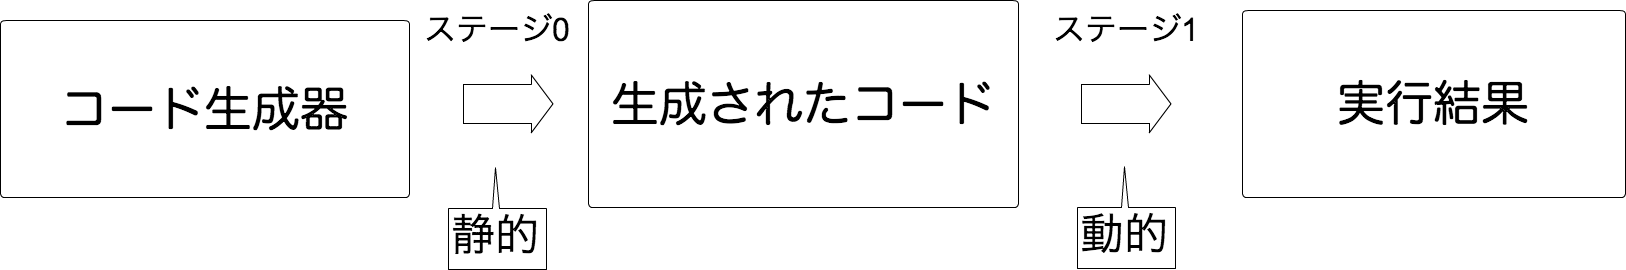
\includegraphics[clip,height=2cm]{./img/prggen.png}

  \begin{itemize}
    % \item コード生成ステージとコード実行ステージ
    % \item 生成前の段階で,生成後のコードの安全性を保証する
  \item コード生成をサポートするプログラム言語(=\alert{コード生成言語})
  %\item[◯]<2-> 生成するプログラムだけでなく,生成されたプログラムも型の整合性が静的に (生成前に) 保証される
  \end{itemize}
\end{frame}

\subsection{コード生成の例}
\begin{frame}
  \frametitle{コード生成言語による記述例}

  \begin{align*}
    \visible<1->{\text{コード生成器}} \visible<1->{&\too \text{生成されるコード}} \\
    \visible<2->{(\cint~ 3)} \visible<2->{&\too \code{3}} \\
    \visible<2->{(\cint~ 3)~ \cPlus~ (\cint~ 5)} \visible<2->{&\too \code{3 + 5}} \\
    \visible<2->{\cfun{x}{~x~ \cPlus~ (\cint~ 3)}} \visible<2->{&\too \code{\fun{x'}{x' + 3}}} \\
    \visible<2->{\cfordo{x = \cdots}{\cdots}~ \cdots}
    \visible<2->{&\too \code{\fordo{x' = \cdots}{\cdots}~ \cdots}}
  \end{align*}

  \begin{visibleenv}<3>
    \begin{exampleblock}{コードコンビネータ}
      \begin{itemize}
      \item 下線つきの演算子
      \item コードを引数にとり,コードを返す
      \end{itemize}
    \end{exampleblock}
  \end{visibleenv}

  % \begin{align*}
  %   \fix f = f (\fix f) \\
  %   \cfordo{x = n}{m}~ e \to \code{\fordo{x = n}{m}~ e}
  % \end{align*}
\end{frame}


\begin{frame}
  \frametitle{power関数のコード生成器}
  \begin{onlyenv}<1>
    普通のpower関数
    \begin{align*}
      \text{~~~~~~power} =~ &\lam x. \fix~ \lam f. \lam n. \\
                            &~~\iif~ n=0~ \then~  1 \\
                            &~~\eelse~ x~ \times~ (f~ (n - 1))
    \end{align*}
  \end{onlyenv}

  \begin{onlyenv}<2->
    \texttt{gen\_power}: powerコード生成器
    \begin{align*}
      \text{gen\_power} =~ &\clam x. \fix~ \lam f. \lam n. \\
                           &~~\iif~ n=0~ \then~ (\cint~ 1) \\
                           &~~\eelse~ x~ \cTimes~ (f~ (n - 1))
    \end{align*}
  \end{onlyenv}

  \pause
  \pause
  $n = 5$に特化したコード生成:
  \pause
  \begin{align*}
    \cfun{x}{~\text{gen\_power}~ x~ 5} \too \code{\fun{x'}{~x'
    \times x' \times x' \times x' \times x' \times 1}}
  \end{align*}

  \center
  \begin{itemize}
  \item power 関数より高速
  \end{itemize}

\end{frame}

% \begin{frame}
%   \frametitle{従来研究}
%   \begin{itemize}
%   \item コード生成プログラムが,安全なコードのみを生成する事を静的に保証
%     %   \item<2-> let挿入等を実現する\alert{計算エフェクトを含む場合の安全性保証の研究は未整備}
%   \item 安全なコード: 構文,型,変数束縛が正しいプログラム
%   \end{itemize}

%   \pause

%   しかし\alert{多段階let挿入}等を実現する\alert{計算エフェクト}を含む場合のコード生成の安全性保証は研究途上
% \end{frame}

% 多段階let挿入というのはあるlet式をn個以上の束縛を抜けて任意の場所へ挿入するということ.
%
% 実際にはtの値によって挿入したい箇所が変わってくる.
% tの値によっては安全じゃない場合があるので,それは型が付かないようにしたい.
% そのような型による項の安全性を考えたい

\begin{frame}[fragile]
  \frametitle{二重forループのコード生成器}
  コード生成器
  \begin{align*}
    & \cfordo{x = (\cint~0)}{(\cint~n)} \\
    & ~~\cfordo{y = (\cint~0)}{(\cint~m)} \\
    & ~~~~~~\caryset{a}{(x,y)}{\text{complex calculation}}
  \end{align*}

  \begin{visibleenv}<2>
    \begin{center}
      \LARGE \downtoo
    \end{center}
    生成されるコード
    \begin{align*}
      &\cbra~ \fordo{x' = 0}{n} \\
      & ~~~~\fordo{y' = 0}{m} \\
      & ~~~~~~\aryset{a}{x',y'}{\text{complex calculation}}~ \cket
    \end{align*}
  \end{visibleenv}
\end{frame}

\begin{frame}
  \frametitle{多段階let挿入の例}
  生成されるコード
  \begin{align*}
    \visible<2->{&\cbra~ \Let ~\blue{w} = \blue{\text{cc1}}~ \In \\}
                 &\visible<1>{\cbra~} \fordo{x' = 0}{n} \\
    \visible<2->{& ~~~~\Let ~\red{u} = \red{\text{cc2}}~ \In \\}
                 & ~~~~\fordo{y' = 0}{m} \\
                 & ~~~~~~\aryset{a}{x',y'}{\visible<2->{\red{u}}~ \visible<1>{\red{\text{cc2}}}} \\
                 & ~~~~~~\aryset{b}{x',y'}{\visible<2->{\blue{w}}~ \visible<1>{\blue{\text{cc1}}}} \cket
  \end{align*}

  \begin{visibleenv}<3>
    \begin{exampleblock}{多段階let挿入}
      \begin{itemize}
      \item 入れ子になったforループなどを飛び越えた\alert{複数のコード移動}を許す仕組み
        % \item ループ不変式の移動等によって,\alert{効率的なコード生成}に必要なプログラミング技法
      \item 効率的なコード生成に必要
      \end{itemize}
    \end{exampleblock}
  \end{visibleenv}
\end{frame}

% \begin{frame}
%   \center
%   \huge{そのような多段階のlet挿入をどうやって行うか}
% \end{frame}

% \begin{frame}
%   \frametitle{多段階let挿入}
%   コード生成器
%   \begin{align*}
%     & \visible<2->{\red{...}~} \cfordo{x = 0}{n} \\
%     & \visible<2->{~~\red{...}~} \cfordo{y = 0}{m} \\
%     & \visible<2->{~~~~\red{...}~} \cLet~u= \text{complex calculation}~\cIn \\
%     & \visible<2->{~~~~~~\red{...}~} (\caryset{\code{a}}{(x,y)}{(i + u)})
%   \end{align*}

%   \begin{onlyenv}<3>
%     \begin{exampleblock}{コントロールオペレータshift0/reset0の導入}
%       $\red{...}$ のところに後に説明する shift0/reset0 というコントロールオペレータを用いることで,多段階let挿入を行う
%     \end{exampleblock}
%   \end{onlyenv}
% \end{frame}

% やりたいことは,このような多段階let挿入をコード生成の前の段階で静的に安全性の保証を行うということ.

\begin{frame}
  \center
  \huge{危険な例}
\end{frame}


\begin{frame}[fragile]
  \frametitle{危険なコード生成の例}
  生成される\red{危険な}コード
  \begin{align*}
    \visible<2->{&\cbra~ \Let ~\blue{w} = \blue{\text{cc1}}~ \In \visible<3->{\footnotesize\magenta{\text{  --- cc1 に x か y が含まれる }}} \\}
                 &\visible<1>{\cbra~} \fordo{x' = 0}{n} \\
    \visible<2->{& ~~~~\Let ~\red{u} = \red{\text{cc2}}~ \In \visible<3->{\footnotesize\magenta{\text{  --- cc2 に y が 含まれる }}} \\}
                 & ~~~~\fordo{y' = 0}{m} \\
                 & ~~~~~~\aryset{a}{x',y'}{\visible<2->{\red{u}}~ \visible<1>{\red{\text{cc2}}}} \\
                 & ~~~~~~\aryset{b}{x',y'}{\visible<2->{\blue{w}}~ \visible<1>{\blue{\text{cc1}}}} \cket
  \end{align*}

  \begin{visibleenv}<4>
    \begin{itemize}
    \item 安全に挿入できる場所とそうでない場所がある
    \end{itemize}
  \end{visibleenv}
\end{frame}


% \begin{frame}
%   \frametitle{危険な例}
%   \begin{align*}
%     & \fordo{i = 0}{n} \\
%     & ~~\fordo{j = 0}{m} \\
%     & ~~~~\magenta{\Let ~y ~= ~a[i] + b[j] ~\In} ~~\tiny{\text{--- t がi,j に依存した式 }} \\
%     & ~~~~~~\aryset{a}{i,j}{b[i] + y} \\
%   \end{align*}

%   \begin{invisibleenv}<1>
%     \begin{center}
%       多段階let挿入\\
%       $\Downarrow$
%     \end{center}
%     \begin{align*}
%       & \magenta{\Let ~y ~= ~a[i] + b[j] ~\In} ~~\tiny{\text{--- t がi,j に依存した式 }} \\
%       & ~~\fordo{i = 0}{n} \\
%       & ~~~~\fordo{j = 0}{m} \\
%       & ~~~~~~\aryset{a}{i,j}{b[i] + y} \\
%     \end{align*}
%   \end{invisibleenv}

%   \begin{onlyenv}<2>
%     \begin{center}
%       多段階let挿入\\
%       $\Downarrow$
%     \end{center}
%     \begin{align*}
%       & \magenta{\Let ~y ~= ~a[i] + b[j] ~\In} \\
%       & ~~\fordo{i = 0}{n} \\
%       & ~~~~\fordo{j = 0}{m} \\
%       & ~~~~~~\aryset{a}{i,j}{b[i] + y} \\
%     \end{align*}
%   \end{onlyenv}
% \end{frame}

\subsection{コード生成の利点と課題}

\begin{frame}
  \frametitle{コード生成の利点と課題}
  利点
  \begin{itemize}
  \item \alert{「保守性・再利用性の高さ」}と\alert{「実行性能の高さ」}の両立
  \end{itemize}

  \pause

  課題
  \begin{itemize}
  \item パラメータに応じて,非常に多数のコードが生成される
    % \item 構文的,意味的に正しくないプログラムを生成しやすい
  \item 生成したコードのデバッグが容易ではない
  \item [⇒] \alert{コード生成の前に安全性を保証}したい
  \end{itemize}
\end{frame}

% \begin{frame}
%   \center
%   \huge{危険なコードは排除したい}
% \end{frame}

\begin{frame}
  \frametitle{コード生成前に型付け,生成後のコードの型安全性を保証}
  \begin{onlyenv}<1>
    \center
    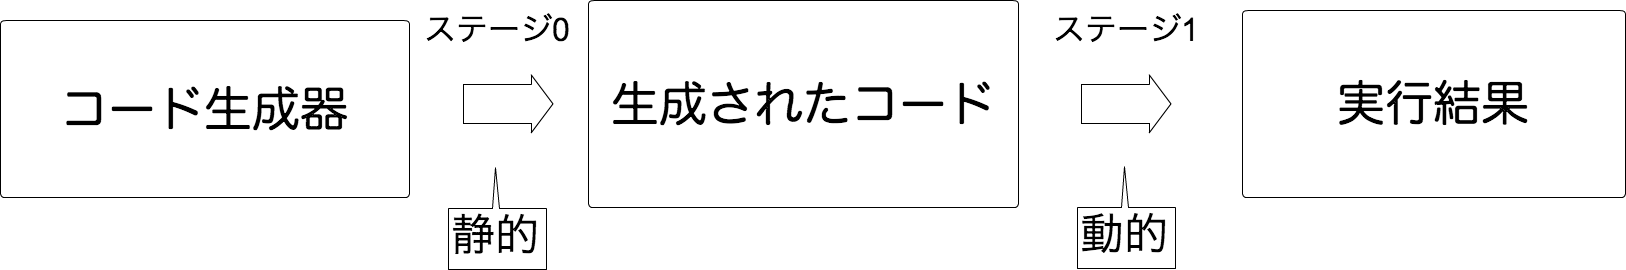
\includegraphics[clip,height=1.9cm]{./img/prggen.png}
  \end{onlyenv}

  \begin{onlyenv}<2>
    \center
    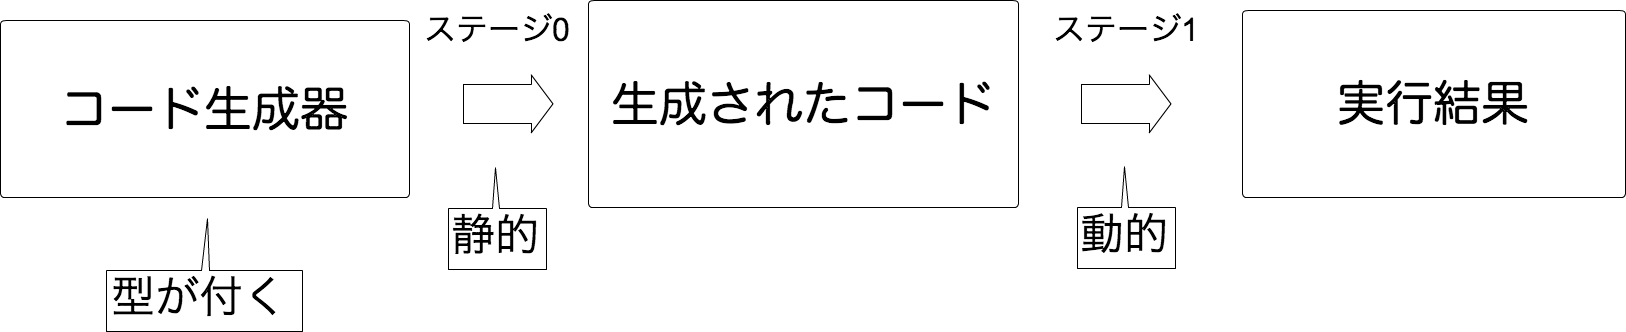
\includegraphics[clip,height=2.4cm]{./img/prggen_type1.png}
  \end{onlyenv}

  \begin{onlyenv}<3>
    \center
    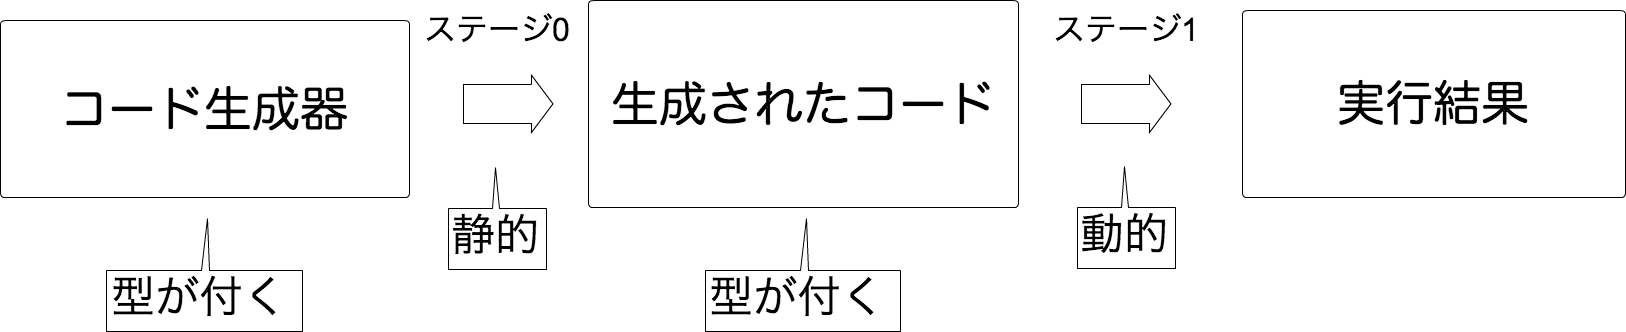
\includegraphics[clip,height=2.4cm]{./img/prggen_type2.png}
  \end{onlyenv}

  \begin{onlyenv}<4>
    \center
    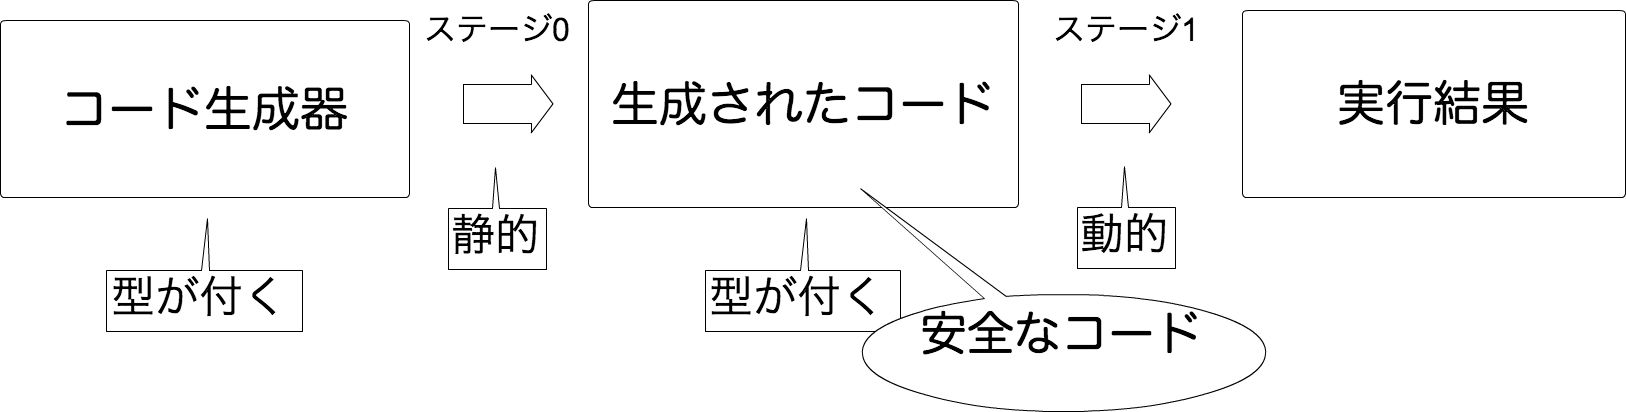
\includegraphics[clip,height=3.0cm]{./img/prggen_type3.png}
  \end{onlyenv}

  \begin{onlyenv}<5>
    \center
    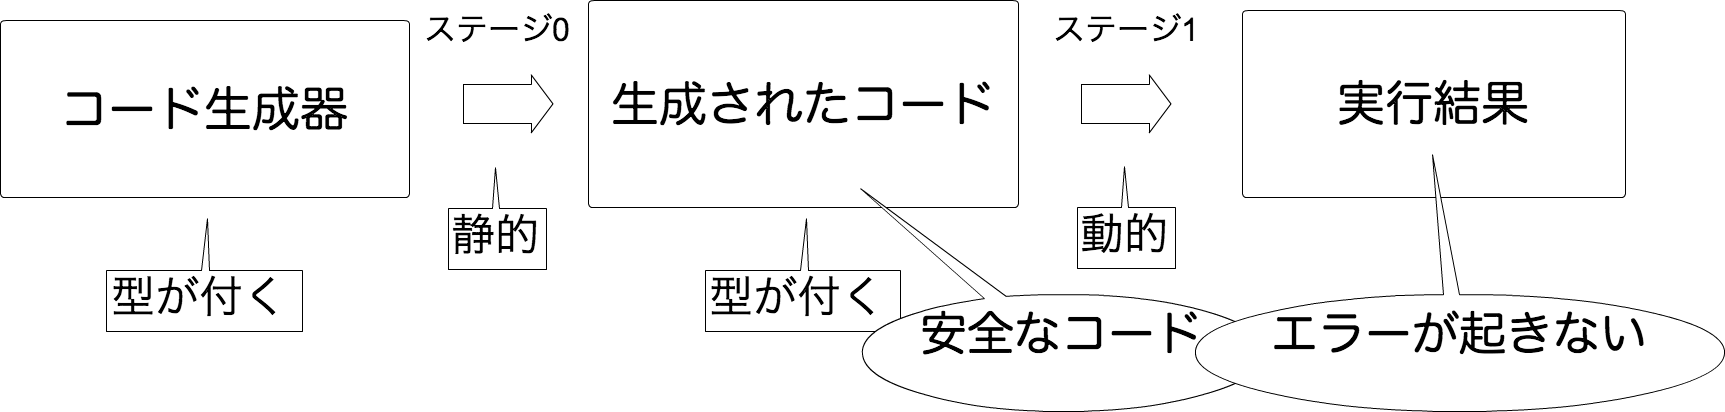
\includegraphics[clip,height=3.0cm]{./img/prggen_type4.png}
  \end{onlyenv}
\end{frame}

% \subsection{限定継続}

% \begin{frame}
%   \frametitle{コントロールオペレータ}
%   \begin{block}{プログラミング言語におけるプログラムを制御するプリミティブ}
%     \begin{itemize}
%     \item exception (例外): C++, Java, ML
%     \item call/cc (第一級継続): Scheme, SML/NJ
%     \item shift/reset (限定継続): Racket, Scala, OCaml
%       \begin{itemize}
%       \item 1989年以降多数研究がある
%       \item コード生成におけるlet挿入が実現可能
%         %       \item shift/reset + コード生成の型システムが幾つか提案されている
%       \end{itemize}
%     \item \alert{shift0/reset0}
%       \begin{itemize}
%       \item 2011年以降研究が活発化.
%       \item コード生成における\alert{多段階let挿入}が可能
%       \end{itemize}
%     \end{itemize}
%   \end{block}
% \end{frame}

%%% Local Variables:
%%% mode: japanese-latex
%%% TeX-master: "slide"
%%% End:
